\section{Experiments}
\label{sec:experiments}

As a first step, we conduct preliminary experiments to justify design choices for our method. Then, in the second part of this section, we compare the localization performances of the proposed image descriptors.

\subsection{Preliminary results}

\subsubsection{Contribution of the depth information}
{
\setlength{\tabcolsep}{5pt}
\renewcommand{\arraystretch}{1.2}
\begin{table}
	\caption{\label{tab/eval_depth} Contribution of the depth side information during training.}
	\scriptsize \center
	\begin{tabular}{ l  c | c  c  c | c  c}
	\multicolumn{2}{c|}{\textbf{Network}} & \multicolumn{3}{c|}{\textbf{Top-1 recall@D}} & \multicolumn{2}{c}{\textbf{Recall@N}} \\	
	           Name & \#Param.  	& @15 & @30 & @50 & @1 & @5\\
	\hline
	RGB + MAC &  2.5M		& 46.7 & 56.7 & 60.9 & 56.3 & 76.6 \\
	RGB$^{+}$ + MAC & 7.9M	& 51.0 & 61.0 & 66.7 & 60.1 &  79.3 \\  
	RGB(D) + MAC &  7.9M	& \textbf{55.9} & \textbf{64.4} & \textbf{67.8} & \textbf{64.0} &  \textbf{80.5} \\
	\hline
	\end{tabular}
\end{table}
}
In this paragraph, we investigate the impact on localization performances provided by the side geometric information on our method. To ensure a fair comparison in terms of number of trainable parameters, we introduce RGB$^+$ network that has the same architecture as our proposed method. We train RGB$^+$ with images only to compare the localization results against our method that uses side depth information. For training RGB$^+$, we simply remove the pixel loss introduced in equation~(\ref{eq:l1_loss}), and make the weights of the decoder $D_a$ trainable when optimizing triplets losses constraints. Results on the validation dataset with encoder architecture Alexnet are presented in table~\ref{tab/eval_depth}.

Increasing the size of the system results in a better localization (RGB$^{+}$ + MAC versus RGB + MAC). However, our RGB(D) + MAC system always produces higher localization results facing RGB$^{+}$ + MAC, which shows that the side depth information provided during training is wisely used to describe the image location.

\subsubsection{Descriptor comparison}
\begin{figure}
	\centering 
	
	\begin{minipage}{0.65\linewidth}		
		\begin{minipage}{0.5\linewidth}
			\includegraphics[width=\linewidth]{plot/mac_vs_vlad/distance}
		\end{minipage}\hfill
		\begin{minipage}{0.5\linewidth}
			\includegraphics[width=\linewidth]{plot/mac_vs_vlad/recall}
		\end{minipage}
		
		\vspace{0.2cm}
		
		\begin{footnotesize}
		\setlength{\tabcolsep}{2pt}
		\begin{tabular}{c l c l c l}
			\textcolor{red}{\Large{- -}} & NetVALD + RGB & \textcolor{blue}{\Large{- -}} & NetVALD + RGB(D)  & \textcolor{magenta}{\Large{- -}} & NetVALD + RGB(H)\\
			\textcolor{red}{\Large{--}} & MAC + RGB & \textcolor{blue}{\Large{--}} & MAC + RGB(D) & \textcolor{magenta}{\Large{--}} & MAC + RGB(H)\\
		\end{tabular}		
		\end{footnotesize}
		
	\end{minipage}\hfill
	\begin{minipage}{0.35\linewidth}
		\caption[Comparison of descriptors pooling layer]{\label{fig:netvlad_vs_mac} \textbf{Comparison of descriptors pooling layer:} NetVLAD~\cite{Arandjelovic2017} pooling layer perform better than MAC~\cite{Razavian2014a} in our preliminary experiment, whatever the tested method.}
	\end{minipage}	
	
\end{figure}

In figure~\ref{fig:netvlad_vs_mac}, we present the localization scores of the three different methods on the validation set with Alexnet as backbone encoder. It clearly demonstrates the superiority of the NetVLAD pooling layer compared to the MAC descriptor. Thus, we only use NetVLAD as pooling layer for the rest of the experiments, in combination with Alexnet or Resnet encoder architecture. Still, this preliminary experiment has shown that the proposed method can be used in combination with various descriptor pooling layers.

\begin{figure}
	\center
	\begin{minipage}{0.16\linewidth}
		\center \scriptsize
		\includegraphics[width=\linewidth]{plot/oxf_cmu/Results_lt_queries/distance}
		
		\includegraphics[width=\linewidth]{plot/oxf_cmu/Results_lt_queries/recall}
		
		a) Oxford -- LT
	\end{minipage}
	\begin{minipage}{0.16\linewidth}
		\center \scriptsize
		\includegraphics[width=\linewidth]{plot/oxf_cmu/Results_snow_queries/distance}	
		
		\includegraphics[width=\linewidth]{plot/oxf_cmu/Results_snow_queries/recall}
				
		b) Oxford -- Snow
	\end{minipage}
	\begin{minipage}{0.16\linewidth}
		\center \scriptsize
		\includegraphics[width=\linewidth]{plot/oxf_cmu/Results_night_queries/distance}	
		
		\includegraphics[width=\linewidth]{plot/oxf_cmu/Results_night_queries/recall}
		
		c) Oxford -- Night
	\end{minipage}
	\begin{minipage}{0.16\linewidth}
		\center \scriptsize
		\includegraphics[width=\linewidth]{plot/oxf_cmu/Results_cmu_lt/distance}	
		
		\includegraphics[width=\linewidth]{plot/oxf_cmu/Results_cmu_lt/recall}
		
		d) CMU -- LT
	\end{minipage}
	\begin{minipage}{0.16\linewidth}
		\center \scriptsize
		\includegraphics[width=\linewidth]{plot/oxf_cmu/Results_cmu_snow/distance}	
		
		\includegraphics[width=\linewidth]{plot/oxf_cmu/Results_cmu_snow/recall}
		
		e) CMU -- Snow
	\end{minipage}
	\begin{minipage}{0.16\linewidth}
		\center \scriptsize
		\includegraphics[width=\linewidth]{plot/oxf_cmu/Results_cmu_autumn/distance}	
		
		\includegraphics[width=\linewidth]{plot/oxf_cmu/Results_cmu_autumn/recall}
		
		f) CMU -- Autumn
	\end{minipage}
	
	\vspace{0.2cm}
	
	\begin{scriptsize}
	\begin{tabular}{c l c l c l c l c l }
		\textcolor{red}{\Large{--}} & Alexnet RGB & 
		\textcolor{red}{\Large{- -}} & Resnet RGB & 
		\textcolor{blue}{\Large{--}} & Alexnet RGB(D) (our) &
		\textcolor{blue}{\Large{- -}} & Resnet RGB(D) (our) &  
		\textcolor{magenta}{\Large{--}} & Alexnet RGB(H)  \\
	\end{tabular}		
	\end{scriptsize}
	
	\caption[Comparison of our method versus competitors]{\label{fig:results} \textbf{Comparison of our method RGB(D) versus hallucination network RGB(H) and networks trained with only images RGB}: we report results for backbone network encoder Resnet (- -) and Alexnet (--). Our method (\textcolor{blue}{in blue}) is superior in every scenario facing hallucination network (\textcolor{magenta}{in magenta}). It also beats, with a significant margin, networks trained with only images (\textcolor{red}{in red}). All the methods failed on the very challenging night to day scenario (b). Curves best viewed in colors.}
\end{figure}

\subsection{Localization results}
\label{subsec:results}

Localization results on the six query sets are presented in figure~\ref{fig:results}. We also show, in figure~\ref{fig:im_exs} ($3^{rd}$, $5^{th}$ and $6^{th}$ columns), some examples of top-1 returned candidate by the different descriptors. Both methods trained with auxiliary depth information (hallucination RGB(H) and our RGB(D)) perform on average better than the RGB baseline. This shows that the geometric clues given during the training process can be efficiently used for the task of image-only retrieval for localization. Compared to hallucination network, our method shows better results, both in terms of recall and precision. We report results for the hallucination network only with encoder Alexnet as we were not able to obtain stable training when using a deeper architecture.

We obtain convincing localization results for the CMU query sets (figure~\ref{fig:results} d-f). It means that our method is able to generalize well on unseen architectural structures for the depth map creation and the extraction of discriminative clue for localization.

Our method shows the best localization improvement on the Oxford - Snow query sets (figure~\ref{fig:results}-b) and CMU -- Snow (for encoder Alexnet, see figure~\ref{fig:results}-e). Standard image descriptors are confused by local changes caused by the snow on the scene whereas our descriptor remains confident by reconstructing the geometric structure of the scene (see figure~\ref{fig:im_exs}, CMU-Snow 1$^{st}$ row). Similar results should be intended regarding Oxford -- Night query set (figure~\ref{fig:results}-c), however our proposal is not able to improve localization accuracy for this particular scenario. We investigate the night to day localization problem specifically in the following section.

\begin{figure}
	\centering
	
	\begin{minipage}{0.02\textwidth}
		\rotatebox{90}{Oxford - LT~~~~~~}
	\end{minipage}\hfill
	\begin{minipage}{0.98\textwidth}
		\centering
		
		{\scriptsize
		\newcolumntype{Y}{>{\centering\arraybackslash}X}
		\begin{tabularx}{0.96\linewidth}{Y Y Y Y Y Y}
		Image & \textbf{RGB(DR)} & \textbf{RGB(D)} & \textbf{RGB(R)} & \multirow{2}{*}{\textbf{RGB(H)}} & \multirow{2}{*}{\textbf{RGB}} \\
		query									  & (our)     &(our)    & (our)    & & \\
		\end{tabularx}}

		\adjincludegraphics[width=0.16\linewidth, trim={0 {.25\height} 0 0}, clip]{plot/oxf_cmu/Results_lt_queries/selected/q213_000011111/request}\hfill
		\adjincludegraphics[width=0.16\linewidth, trim={0 {.25\height} 0 0}, clip, cfbox=green 1pt -1pt]{plot/oxf_cmu/Results_lt_queries/selected/q213_000011111/0_3_DR_R_VLAD_MATCH}\hfill
		\adjincludegraphics[width=0.16\linewidth, trim={0 {.25\height} 0 0}, clip, cfbox=green 1pt -1pt]{plot/oxf_cmu/Results_lt_queries/selected/q213_000011111/0_2_D_R_VLAD_MATCH}\hfill
		\adjincludegraphics[width=0.16\linewidth, trim={0 {.25\height} 0 0}, clip, cfbox=green 1pt -1pt]{plot/oxf_cmu/Results_lt_queries/selected/q213_000011111/0_2_R_R_VLAD_MATCH}\hfill
		\adjincludegraphics[width=0.16\linewidth, trim={0 {.25\height} 0 0}, clip, cfbox=red 1pt -1pt]{plot/oxf_cmu/Results_lt_queries/selected/q213_000011111/0_1_H_A_VLAD_NO}\hfill
		\adjincludegraphics[width=0.16\linewidth, trim={0 {.25\height} 0 0}, clip, cfbox=red 1pt -1pt]{plot/oxf_cmu/Results_lt_queries/selected/q213_000011111/0_0_R_VLAD_PCA_NO}
		
		\adjincludegraphics[width=0.16\linewidth, trim={0 {.25\height} 0 0}, clip]{plot/oxf_cmu/Results_lt_queries/selected/q138_001000100/request}\hfill
		\adjincludegraphics[width=0.16\linewidth, trim={0 {.25\height} 0 0}, clip, cfbox=red 1pt -1pt]{plot/oxf_cmu/Results_lt_queries/selected/q138_001000100/0_3_DR_R_VLAD_NO}\hfill
		\adjincludegraphics[width=0.16\linewidth, trim={0 {.25\height} 0 0}, clip, cfbox=red 1pt -1pt]{plot/oxf_cmu/Results_lt_queries/selected/q138_001000100/0_2_D_R_VLAD_NO}\hfill
		\adjincludegraphics[width=0.16\linewidth, trim={0 {.25\height} 0 0}, clip, cfbox=green 1pt -1pt]{plot/oxf_cmu/Results_lt_queries/selected/q138_001000100/0_2_R_R_VLAD_MATCH}\hfill
		\adjincludegraphics[width=0.16\linewidth, trim={0 {.25\height} 0 0}, clip, cfbox=red 1pt -1pt]{plot/oxf_cmu/Results_lt_queries/selected/q138_001000100/0_1_H_A_VLAD_MATCH}\hfill
		\adjincludegraphics[width=0.16\linewidth, trim={0 {.25\height} 0 0}, clip, cfbox=red 1pt -1pt]{plot/oxf_cmu/Results_lt_queries/selected/q138_001000100/0_0_R_VLAD_PCA_NO}
		
	\end{minipage}
	
	\begin{minipage}{0.02\textwidth}
		\rotatebox{90}{Oxford - Snow}
	\end{minipage}\hfill
	\begin{minipage}{0.98\textwidth}
		\centering
		
		\adjincludegraphics[width=0.16\linewidth, trim={0 {.25\height} 0 0}, clip]{plot/oxf_cmu/Results_snow_queries/selected/q61_000000001/request}\hfill
		\adjincludegraphics[width=0.16\linewidth, trim={0 {.25\height} 0 0}, clip, cfbox=green 1pt -1pt]{plot/oxf_cmu/Results_snow_queries/selected/q61_000000001/0_3_DR_R_VLAD_MATCH}\hfill
		\adjincludegraphics[width=0.16\linewidth, trim={0 {.25\height} 0 0}, clip, cfbox=red 1pt -1pt]{plot/oxf_cmu/Results_snow_queries/selected/q61_000000001/0_2_D_R_VLAD_NO}\hfill	
		\adjincludegraphics[width=0.16\linewidth, trim={0 {.25\height} 0 0}, clip, cfbox=red 1pt -1pt]{plot/oxf_cmu/Results_snow_queries/selected/q61_000000001/0_2_R_R_VLAD_NO}\hfill	
		\adjincludegraphics[width=0.16\linewidth, trim={0 {.25\height} 0 0}, clip, cfbox=red 1pt -1pt]{plot/oxf_cmu/Results_snow_queries/selected/q61_000000001/0_1_H_A_VLAD_NO}\hfill	
		\adjincludegraphics[width=0.16\linewidth, trim={0 {.25\height} 0 0}, clip, cfbox=red 1pt -1pt]{plot/oxf_cmu/Results_snow_queries/selected/q61_000000001/0_0_R_VLAD_PCA_NO}
		
		\adjincludegraphics[width=0.16\linewidth, trim={0 {.25\height} 0 0}, clip]{plot/oxf_cmu/Results_snow_queries/selected/q86_000010001/request}\hfill
		\adjincludegraphics[width=0.16\linewidth, trim={0 {.25\height} 0 0}, clip, cfbox=green 1pt -1pt]{plot/oxf_cmu/Results_snow_queries/selected/q86_000010001/0_3_DR_R_VLAD_MATCH}\hfill
		\adjincludegraphics[width=0.16\linewidth, trim={0 {.25\height} 0 0}, clip, cfbox=green 1pt -1pt]{plot/oxf_cmu/Results_snow_queries/selected/q86_000010001/0_2_D_R_VLAD_MATCH}\hfill
		\adjincludegraphics[width=0.16\linewidth, trim={0 {.25\height} 0 0}, clip, cfbox=red 1pt -1pt]{plot/oxf_cmu/Results_snow_queries/selected/q86_000010001/0_2_R_R_VLAD_NO}\hfill
		\adjincludegraphics[width=0.16\linewidth, trim={0 {.25\height} 0 0}, clip, cfbox=red 1pt -1pt]{plot/oxf_cmu/Results_snow_queries/selected/q86_000010001/0_1_H_A_VLAD_NO}\hfill
		\adjincludegraphics[width=0.16\linewidth, trim={0 {.25\height} 0 0}, clip, cfbox=red 1pt -1pt]{plot/oxf_cmu/Results_snow_queries/selected/q86_000010001/0_0_R_VLAD_PCA_NO}
		
	\end{minipage}

	\begin{minipage}{0.02\textwidth}
		\rotatebox{90}{CMU - LT}
	\end{minipage}\hfill
	\begin{minipage}{0.98\textwidth}
		\centering
		
		\includegraphics[width=0.16\linewidth]{plot/oxf_cmu/Results_cmu_lt/selected/q119_000101001/request}\hfill
		\includegraphics[width=0.16\linewidth, cfbox=green 1pt -1pt]{plot/oxf_cmu/Results_cmu_lt/selected/q119_000101001/0_3_DR_R_VLAD_MATCH}\hfill
		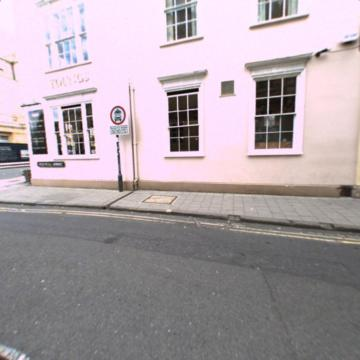
\includegraphics[width=0.16\linewidth, cfbox=red 1pt -1pt]{plot/oxf_cmu/Results_cmu_lt/selected/q119_000101001/0_2_D_R_VLAD_NO}\hfill	
		\includegraphics[width=0.16\linewidth, cfbox=red 1pt -1pt]{plot/oxf_cmu/Results_cmu_lt/selected/q119_000101001/0_2_R_R_VLAD_NO}\hfill	
		\includegraphics[width=0.16\linewidth, cfbox=red 1pt -1pt]{plot/oxf_cmu/Results_cmu_lt/selected/q119_000101001/0_1_H_A_VLAD_NO}\hfill	
		\includegraphics[width=0.16\linewidth, cfbox=red 1pt -1pt]{plot/oxf_cmu/Results_cmu_lt/selected/q119_000101001/0_0_R_VLAD_PCA_NO}
		
		\includegraphics[width=0.16\linewidth]{plot/oxf_cmu/Results_cmu_lt/selected/q1413_000110000/request}\hfill
		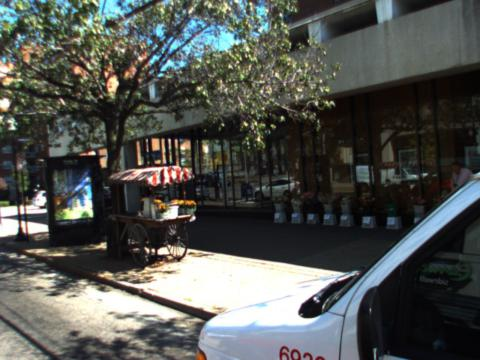
\includegraphics[width=0.16\linewidth, cfbox=red 1pt -1pt]{plot/oxf_cmu/Results_cmu_lt/selected/q1413_000110000/0_3_DR_R_VLAD_NO}\hfill
		\includegraphics[width=0.16\linewidth, cfbox=green 1pt -1pt]{plot/oxf_cmu/Results_cmu_lt/selected/q1413_000110000/0_2_D_R_VLAD_MATCH}\hfill
		\includegraphics[width=0.16\linewidth, cfbox=red 1pt -1pt]{plot/oxf_cmu/Results_cmu_lt/selected/q1413_000110000/0_2_R_R_VLAD_NO}\hfill
		\includegraphics[width=0.16\linewidth, cfbox=red 1pt -1pt]{plot/oxf_cmu/Results_cmu_lt/selected/q1413_000110000/0_1_H_A_VLAD_NO}\hfill
		\includegraphics[width=0.16\linewidth, cfbox=red 1pt -1pt]{plot/oxf_cmu/Results_cmu_lt/selected/q1413_000110000/0_0_R_VLAD_PCA_NO}
		
	\end{minipage}
	
	\begin{minipage}{0.02\textwidth}
		\rotatebox{90}{CMU - Snow}
	\end{minipage}\hfill
	\begin{minipage}{0.98\textwidth}
		\centering
		
		\includegraphics[width=0.16\linewidth]{plot/oxf_cmu/Results_cmu_snow/selected/q847_000010001/request}\hfill
		\includegraphics[width=0.16\linewidth, cfbox=green 1pt -1pt]{plot/oxf_cmu/Results_cmu_snow/selected/q847_000010001/0_3_DR_R_VLAD_MATCH}\hfill
		\includegraphics[width=0.16\linewidth, cfbox=green 1pt -1pt]{plot/oxf_cmu/Results_cmu_snow/selected/q847_000010001/0_2_D_R_VLAD_MATCH}\hfill	
		\includegraphics[width=0.16\linewidth, cfbox=red 1pt -1pt]{plot/oxf_cmu/Results_cmu_snow/selected/q847_000010001/0_2_R_R_VLAD_NO}\hfill	
		\includegraphics[width=0.16\linewidth, cfbox=red 1pt -1pt]{plot/oxf_cmu/Results_cmu_snow/selected/q847_000010001/0_1_H_A_VLAD_NO}\hfill	
		\includegraphics[width=0.16\linewidth, cfbox=red 1pt -1pt]{plot/oxf_cmu/Results_cmu_snow/selected/q847_000010001/0_0_R_VLAD_PCA_NO}
		
		\includegraphics[width=0.16\linewidth]{plot/oxf_cmu/Results_cmu_snow/selected/q543_000010101/request}\hfill
		\includegraphics[width=0.16\linewidth, cfbox=green 1pt -1pt]{plot/oxf_cmu/Results_cmu_snow/selected/q543_000010101/0_3_DR_R_VLAD_MATCH}\hfill
		\includegraphics[width=0.16\linewidth, cfbox=green 1pt -1pt]{plot/oxf_cmu/Results_cmu_snow/selected/q543_000010101/0_2_D_R_VLAD_MATCH}\hfill
		\includegraphics[width=0.16\linewidth, cfbox=green 1pt -1pt]{plot/oxf_cmu/Results_cmu_snow/selected/q543_000010101/0_2_R_R_VLAD_MATCH}\hfill
		\includegraphics[width=0.16\linewidth, cfbox=red 1pt -1pt]{plot/oxf_cmu/Results_cmu_snow/selected/q543_000010101/0_1_H_A_VLAD_NO}\hfill
		\includegraphics[width=0.16\linewidth, cfbox=red 1pt -1pt]{plot/oxf_cmu/Results_cmu_snow/selected/q543_000010101/0_0_R_VLAD_PCA_NO}
		
	\end{minipage}
	
	\begin{minipage}{0.02\textwidth}
		\rotatebox{90}{CMU - Autumn}
	\end{minipage}\hfill
	\begin{minipage}{0.98\textwidth}
		\centering
		
		\includegraphics[width=0.16\linewidth]{plot/oxf_cmu/Results_cmu_autumn/selected/q865_000010001/request}\hfill
		\includegraphics[width=0.16\linewidth, cfbox=green 1pt -1pt]{plot/oxf_cmu/Results_cmu_autumn/selected/q865_000010001/0_3_DR_R_VLAD_MATCH}\hfill
		\includegraphics[width=0.16\linewidth, cfbox=green 1pt -1pt]{plot/oxf_cmu/Results_cmu_autumn/selected/q865_000010001/0_2_D_R_VLAD_MATCH}\hfill
		\includegraphics[width=0.16\linewidth, cfbox=red 1pt -1pt]{plot/oxf_cmu/Results_cmu_autumn/selected/q865_000010001/0_2_R_R_VLAD_NO}\hfill	
		\includegraphics[width=0.16\linewidth, cfbox=red 1pt -1pt]{plot/oxf_cmu/Results_cmu_autumn/selected/q865_000010001/0_1_H_A_VLAD_NO}\hfill	
		\includegraphics[width=0.16\linewidth, cfbox=red 1pt -1pt]{plot/oxf_cmu/Results_cmu_autumn/selected/q865_000010001/0_0_R_VLAD_PCA_NO}
		
		\includegraphics[width=0.16\linewidth]{plot/oxf_cmu/Results_cmu_autumn/selected/q267_000010101/request}\hfill
		\includegraphics[width=0.16\linewidth, cfbox=green 1pt -1pt]{plot/oxf_cmu/Results_cmu_autumn/selected/q267_000010101/0_3_DR_R_VLAD_MATCH}\hfill
		\includegraphics[width=0.16\linewidth, cfbox=green 1pt -1pt]{plot/oxf_cmu/Results_cmu_autumn/selected/q267_000010101/0_2_D_R_VLAD_MATCH}\hfill
		\includegraphics[width=0.16\linewidth, cfbox=green 1pt -1pt]{plot/oxf_cmu/Results_cmu_autumn/selected/q267_000010101/0_2_R_R_VLAD_MATCH}\hfill
		\includegraphics[width=0.16\linewidth, cfbox=red 1pt -1pt]{plot/oxf_cmu/Results_cmu_autumn/selected/q267_000010101/0_1_H_A_VLAD_NO}\hfill
		\includegraphics[width=0.16\linewidth, cfbox=red 1pt -1pt]{plot/oxf_cmu/Results_cmu_autumn/selected/q267_000010101/0_0_R_VLAD_PCA_NO}
		
	\end{minipage}
	
	\caption[Comparison of top-1 retrieved images]{\label{fig:im_exs} \textbf{Comparison of top-1 retrieved images}: we show top-1 retrieved candidate after the nearest neighbor search for the different descriptor. \textcolor{red}{Red} box indicates a wrong match and \textcolor{green}{green} box a proper one (\textit{i.e.} retrieved image lies in 25m radius from the query ground truth position). All the descriptor use Resnet18 as backbone, excepted RGB(H).}
	
\end{figure}